%%%%%%%%%%%%%%%%%%%%%%% file template.tex %%%%%%%%%%%%%%%%%%%%%%%%%
%
% This is a general template file for the LaTeX package SVJour3
% for Springer journals.          Springer Heidelberg 2010/09/16
%
% Copy it to a new file with a new name and use it as the basis
% for your article. Delete % signs as needed.
%
% This template includes a few options for different layouts and
% content for various journals. Please consult a previous issue of
% your journal as needed.
%
%%%%%%%%%%%%%%%%%%%%%%%%%%%%%%%%%%%%%%%%%%%%%%%%%%%%%%%%%%%%%%%%%%%
%
% First comes an example EPS file -- just ignore it and
% proceed on the \documentclass line
% your LaTeX will extract the file if required
\begin{filecontents*}{example.eps}
%!PS-Adobe-3.0 EPSF-3.0
%%BoundingBox: 19 19 221 221
%%CreationDate: Mon Sep 29 1997
%%Creator: programmed by hand (JK)
%%EndComments
gsave
newpath
  20 20 moveto
  20 220 lineto
  220 220 lineto
  220 20 lineto
closepath
2 setlinewidth
gsave
  .4 setgray fill
grestore
stroke
grestore
\end{filecontents*}
%
\RequirePackage{fix-cm}
%
%\documentclass{svjour3}                     % onecolumn (standard format)
\documentclass[smallcondensed]{svjour3}     % onecolumn (ditto)
%\documentclass[smallextended]{svjour3}       % onecolumn (second format)
%\documentclass[twocolumn]{svjour3}          % twocolumn
%
\smartqed  % flush right qed marks, e.g. at end of proof
%
%\usepackage{mathptmx}      % use Times fonts if available on your TeX system
\usepackage{newtxtext,newtxmath}      % use Times fonts if available on your TeX system
%
% insert here the call for the packages your document requires
%\usepackage{latexsym}
%
\usepackage{amsmath}
\usepackage{amssymb}
\usepackage{algorithm}
\usepackage{pgfplots}
\usepackage{graphicx}
\usepackage{calc}
\usepackage{mathtools}
\usepackage{color}
\usepackage[inline]{enumitem}
\usepackage{float}
\usepackage{xfrac}
\usepackage[hidelinks]{hyperref}
\usepackage[capitalize, noabbrev]{cleveref}
\usepackage{algpseudocode}
\usepackage{longtable}
\usepackage{booktabs}
\usepackage{xspace}
\usepackage{manfnt}
\usepackage{siunitx}
\usepackage{float}

\usetikzlibrary{matrix}
\usepgfplotslibrary{groupplots}
\newfloat{algorithm}{t}{lop}

\definecolor{tol/contrast/blue}{RGB}{0,68,136}
\definecolor{tol/contrast/red}{RGB}{187,85,102}
\definecolor{tol/contrast/yellow}{RGB}{221,170,51}

\definecolor{tol/vibrant/blue}{RGB}{0,119,187}
\definecolor{tol/vibrant/cyan}{RGB}{51,187,238}
\definecolor{tol/vibrant/teal}{RGB}{0,153,136}
\definecolor{tol/vibrant/orange}{RGB}{238,119,51}
\definecolor{tol/vibrant/red}{RGB}{204,51,17}
\definecolor{tol/vibrant/magenta}{RGB}{238,51,119}
\definecolor{tol/vibrant/grey}{RGB}{187,187,187}

\definecolor{tol/rainbow/26}{RGB}{220,5,12}
\definecolor{tol/rainbow/18}{RGB}{247,240,86}
\definecolor{tol/rainbow/15}{RGB}{78,178,101}
\definecolor{tol/rainbow/10}{RGB}{25,101,176}

% please place your own definitions here and don't use \def but
% \newcommand{}{}

\newcommand{\titletable}[2]{\bgroup\renewcommand{\arraystretch}{1.0}\begin{tabular}{@{}c@{}}{#1}\\\scalebox{0.75}{$N={#2}$}\end{tabular}\egroup}
\renewcommand{\vec}[1]{\boldsymbol{#1}}

\newcommand{\param}{\theta}
\newcommand{\params}{\vec{\theta}}
\newcommand{\laplacian}{\Delta}
\newcommand{\cross}{\times}
\newcommand{\grad}[1][]{\nabla\if\relax\detokenize{#1}\relax\else{}_{#1}\fi}
\renewcommand{\div}[1][]{\grad[#1]\cdot}
\renewcommand{\d}{\relax\ifnum\lastnodetype>0\mskip\thinmuskip\fi\textnormal{d}}
\renewcommand{\L}{\mathcal{E}}

\newcommand{\domain}{\ensuremath{\Omega}}
\newcommand{\interface}{\ensuremath{\Gamma}}
\newcommand{\archetype}{\ensuremath{\hat{\Gamma}}}
\newcommand{\reference}{\ensuremath{\interface_0}}
\newcommand{\spread}{\ensuremath{\mathcal{S}}}
\newcommand{\interp}{\ensuremath{\mathcal{S}^\dagger}}
\newcommand{\Dirac}{\delta}
\newcommand{\kernel}{\phi}
\newcommand{\basic}{\varphi}
\newcommand{\Basic}{\Phi}
\newcommand{\poly}{p}
\newcommand{\Poly}{P}

\newcommand{\x}{\vec{x}}
\newcommand{\X}{\vec{X}}
\renewcommand{\u}{\vec{u}}
\newcommand{\U}{\dot{\vec{X}}}
\newcommand{\f}{\vec{f}}
\newcommand{\F}{\vec{F}}
\newcommand{\um}{\mskip\thinmuskip\si{\micro\meter}}
\newcommand{\dynpercm}{\mskip\thinmuskip\si{dyn\per\centi\meter}}
\newcommand{\us}{\mskip\thinmuskip\si{\micro\second}}
\newcommand{\ms}{\mskip\thinmuskip\si{\milli\second}}

\newcommand{\thrust}{\texttt{thrust}}

% Insert the name of "your journal" with
% \journalname{myjournal}
\journalname{Journal of Scientific Computing}
%
\begin{document}

\title{%
    A fine-grained parallelization of the immersed boundary method
    %\thanks{$thanks$}
}

%\subtitle{}
%\titlerunning{}

\author{Andrew Kassen \and Varun Shankar \and Aaron Fogelson}

\authorrunning{}
%\authorrunning{Short form of author list} % if too long for running head

\institute{%
    A. Kassen \at Department of Mathematics \newline University of Utah \and
    V. Shankar \at School of Computing \newline University of Utah \and
    A. Fogelson \at Department of Mathematics \newline University of Utah \newline
    \email{fogelson@math.utah.edu}
}

\date{Received: date / Accepted: date}
% The correct dates will be entered by the editor


\maketitle

\begin{abstract}
    We introduce a parallel implementation of the immersed boundary method
    interaction operations which relies on the well-studied parallel primitives
    key-value sort and segmented reduce. This makes the algorithms feasible for
    use on general purpose graphical processing units (GPGPUs) in addition to
    most other architectures.

% \keywords{}
% \PACS{}
% \subclass{MSC code1 \and MSC code2 \and more}
\end{abstract}

%\section{Introduction}

Many problems in biophysics involve the interaction of an incompressible fluid and an
immersed elastic interface. The solution to these problems can be approximated using the
immersed boundary (IB) method, which was developed by Charles Peskin to simulate blood
flow through the heart \cite{Peskin:1972wa}. This method couples the equations governing
fluid velocity and pressure to those governing the interface movement and elastic forces
via operations we will refer to as \term{interpolation} and \term{spreading}. We treat
solving the fluid equations and computing elastic forces as an implementation detail and
focus primarily on the interpolation and spreading operations. We are motivated by the
desire to simulate whole blood, composed of red blood cells (RBCs) and platelets immersed
in blood plasma, in a vessel lined by endothelial cells.  Approximately 40\% of the
volume in healthy human blood is occupied by RBCs, and so even small domains may require
tens of thousands of points or more to discretize these cells.

To take advantage of modern computing architectures, with ever increasing numbers of
processors, it is necessary to develop parallel algorithms for the IB method. McQueen and
Peskin present a domain decomposition scheme to parallelize the interpolation and
spreading operations on the Cray C-90 computer with a modest number of vector processors
\cite{McQueen:1997kw}.  Their results illustrate the need for a fast interpolation and
spreading: even parallelized, they spend roughly half of the wall clock time spreading
and interpolating.  However, for a grid of $128^3$ points, their approach is limited to
1024 concurrent threads, and increasing parallelization requires refinement of the
fluid grid. General purpose graphical processing units (GPGPUs), on the other hand,
are capable of running thousands of threads concurrently.

Here, we discuss the parallelization of interpolation and introduce a new parallelization
for the spreading operation. We demonstrate that the concurrency of these algorithms
scales with the number of IB points, independently of the Eulerian grid. The algorithms
divide these operations into trivially parallelizable tasks and parallel primitives. They
are therefore suitable for use on GPGPUs, along with many other architectures. We begin
with an introduction to the IB method, and the role of the interpolation and spreading
operations.

% vim: cc=90 tw=89

%\section{Review of the immersed boundary method}

Consider a $d$-dimensional ($d=2$ or 3) rectangular domain $\domain$, which is filled
with a viscous incompressible fluid with constant viscosity $\mu$ and density $\rho$, and
contains an immersed elastic structure, $\interface$. The structure is impermeable to the
fluid and moves at the local fluid velocity, is deformed by this motion, and imparts a
force to the fluid. Otherwise, the interface is treated as part of the fluid. 

The fluid velocity, $\u = \u(\x,\,t)$, and pressure, $p = p(\x,\,t)$, are governed by the
incompressible Navier-Stokes equations for a Newtonian fluid,
\begin{gather}
    \label{eq:ins-evol}
    \rho(\u_t + \u\cdot\grad\u) = \mu\Delta\u - \grad p + \f, \\
    \label{eq:ins-incomp}
    \div\u = 0,
\end{gather}
where $p$ is the pressure and $\f$ is the elastic force density. This is a set of $d+1$
equations in $d+1$ unknowns: the $d$ components of $\u$, and $p$. The equations are
written relative to the Eulerian frame, so that the coordinates $\x$ are independent
variables. Throughout, we write Eulerian quantities in the lowercase Latin alphabet.

Let $\X=\X(\params,\,t)$ represent a parametrization of the Cartesian coordinates of the
immersed interface with material coordinates $\params$ at time $t$. Let $\L[\X]$ be the
energy density functional for the elastic interface material. The elastic force density
is computed by evaluating the Fréchet derivative of $\L$,
\begin{equation}
    \label{eq:forces}
    \F = -\delta \L[\X],
\end{equation}
where $\delta$ represents the first variation. Uppercase Latin letters represent
Lagrangian quantities and are functions of $\params$ and $t$.

The interface moves at the local fluid velocity, and force balance on the interface
between the interface and fluid dictates that the interface force on the fluid is equal
to the elastic force. Analytically, the fluid-interface interactions can be written
\begin{gather}
    \label{eq:interpolation}
    \U(\params,\,t) = \int_\domain \Dirac(\x-\X(\params,\,t)) \u(\x,\,t)\d\x,\ \text{and} \\
    \label{eq:spreading}
    \f(\x,\,t) = \int_\interface \Dirac(\x-\X(\params,\,t))\F(\params,\,t)\d\params,
\end{gather}
where $\U(\params,\,t)$ represents the derivative of $\X(\params,\,t)$ with respect to
$t$, and $\Dirac(\x-\X(\params,\,t))$ is the Dirac $\Dirac$-function centered at
$\X(\params,\,t)$.  Equation \eqref{eq:interpolation} is called \term{interpolation}, and
the result of the right-hand side is the fluid velocity at $\X(\params,\,t)$; namely,
$\U(\params,\,t) = \u(\X(\params,\,t),\,t)$.  Equation \eqref{eq:spreading} is called
\term{spreading}, because while $\F(\params,\,t)$ has units of force per unit \emph{area}
on $\interface$, $\f(\x,\,t)$ has units of force per unit \emph{volume} in $\domain$. The
force $\F(\params,\,t)\d\params$ over area $\d\params$ is ``spread'' to the force
$\f(\x,\,t)\d\x$ over volume $\d\x$. 

The fluid equations \eqref{eq:ins-evol}--\eqref{eq:ins-incomp} are spatially discretized
on a regular grid of spacing $h$ so that $\domain$ is divided into square or cubic cells
of side length $h$. Because of the checkerboard instability (see, e.g.,
\cite{Wesseling:2001ci}) in solving the Navier-Stokes equations on collocated regular
grids, we stagger the components of Eulerian vector quantities. As a result, different
components are discretized at different locations, but corresponding components are
discretized on the same grid. Grid cells for these staggered grids do not coincide. We
therefore consider each of these grids individually. We use $\domain_h$ to denote the set
of grid points for the grid under consideration, and $n_\omega$ to denote the number of
grid points. The momentum equation \eqref{eq:ins-evol} is discretized in time using a
second-order implicit-explicit Runge-Kutta method \cite{Peskin:2002go}, and the
incompressibility condition \eqref{eq:ins-incomp} is satisfied using PmIII
\cite{Brown:2001bq}.

The Lagrangian force density \ref{eq:forces} is evaluated at a set of points, usually a
\emph{fixed} set of points in material coordinates, referred to as IB points. The
notation $\X_j=\X(\params_j,\,t)$ refers to an individual IB point on $\interface$ in
Cartesian coordinates. The typical heuristic for distributing the points $\X_j$ on a
connected interface places neighboring IB points at most $h$ apart from one another, and
often at most $h/2$ apart. We therefore denote the set of IB points by $\interface_h$ and
the number of IB points by $n_\gamma$. From these points, we construct a smooth
approximation to the interface using radial basis functions \cite{Shankar:2015km}. This
allows us to calculate geometric properties using well-known formulas, and evaluate the
forces \eqref{eq:forces} analytically \cite{Maxian:2018ek}.

The singular integrals \eqref{eq:interpolation} and \eqref{eq:spreading} do not lend
themselves easily to evaluation. In particular, it is unlikely that IB points and grid
points will coincide. For a regular grid with spacing $h$, we replace the Dirac
$\Dirac$-function with a regularized kernel, $\Dirac_h$, which is a product of
one-dimensional kernels, $h^{-1}\kernel(h^{-1}x)$. There are several options for
$\kernel$ \cite{Griffith:2020hi}, but we will restrict ourselves to the simple cosine
kernel \cite{Peskin:2002go}.

Let $\domain_h$ be one of the Eulerian grids for vector-valued quantities. Discretizing
equations \eqref{eq:scalar-interp} and \eqref{eq:scalar-spread} on $\domain_h$ and
$\interface_h$, respectively, yields
\begin{align}
    \label{eq:disc-interp}
    \dot{X}^n_j &= \sum_i \delta_h(\x_i-\X^n_j)u^n_i h^d \quad \text{and} \\
    \label{eq:disc-spread}
    f^n_i &= \sum_j \delta_h(\x_i-\X^n_j)F^n_j \d\theta_j,
\end{align}
where $u^n_i$ and $f^n_i$ are discrete approximations to the components of $\u$ and $\f$
at $\x_i\in\domain_h$ and time $t=t_n$, and $\dot{X}^n_{\smash j}$ and $F^n_{\smash j}$
are their Lagrangian counterparts at $\X_{\smash j}$, respectively. The terms $h^d$ and
$\d\theta_{\smash j}$ are integration weights analogous to $\d\x$ and $\d\params$. Each
of the above equations look like a matrix-vector multiplication, so we define the
\emph{spreading matrix} $\spread=(\delta_h(\x_i-\X^n_{\smash j}))$ with row $i$ and
column $j$. We call its transpose, $\interp$, the \emph{interpolation matrix}. Collecting
values $u^n_ih^d$ as $\u^n$ at each grid point and $F^n_{\smash j}\d\theta_{\smash j}$ as
$\F^n$ at each IB point, we rewrite Equations \eqref{eq:disc-interp} and
\eqref{eq:disc-spread} in matrix form as
\begin{align}
    \label{eq:matrix-interp}
    \dot{\X}^n &= \interp\u^n \quad\text{and} \\
    \label{eq:matrix-spread}
    \f^n &= \spread\F^n,
\end{align}
respectively.

Collectively, the equations \eqref{eq:ins-evol}--\eqref{eq:spreading} constitute the
IB method, and while different implementations depend on myriad details, a single step
proceeds with timestep $k$ roughly as follows:
\begin{enumerate}[label=(\texttt{\alph*})]
    \item interpolate $\u^n$ to $\X^n$ to get $\U^\ast$,
    \item predict Lagrangian positions $\X^\ast = \X^n + k\U^\ast$,
    \item compute Lagrangian forces $\F^\ast$ using positions $\X^\ast$,
    \item spread $-\F^\ast$ from $\X^\ast$ to get $\f^\ast$,
    \item solve for updated Eulerian velocities $\u^\ast$,
    \item project $\u^\ast$ into space of divergence-free vector fields to get
        $\u^{n+1}$,
    \item interpolate $\u^{n+1}$ to $\X^n$ to get $\U^{n+1}$, and
    \item update $\X^{n+1} = \X^n + k \U^{n+1}$.
\end{enumerate}
We group these steps into 3 categories: the purely Eulerian (\texttt{e}) and
(\texttt{f}); the purely Lagrangian (\texttt{b}), (\texttt{c}), and (\texttt{h}); and the
Eulerian-Lagrangian coupling (\texttt{a}), (\texttt{d}), and (\texttt{g}). We discuss the
%parallelization of the
first two categories \textcolor{red}{in a forthcoming paper}.
%
%briefly before tackling the third.
%
%\section{Parallelization in the Eulerian and Lagrangian frames}
%
%Given an Eulerian force density $\f$ and Lagrangian fluid velocity $\U$ it is
%a straightforward matter to parallelize the evolution of the fluid velocity and interface
%forces, as they are otherwise independent of one another. Assuming fixed sets of grid
%points and material coordinates for IB points, any interdependence of points within a
%frame can be accounted for at the outset to ease parallelization during the course of a
%simulation.
%
%To solve for the fluid velocity, we use the 2nd-order Runge-Kutta method described in
%\cite{Peskin:2002go}.  We compute the advection term in conservation form. For, e.g., the
%quantity $(uv)_y$, we average $u$ in the $y$ direction and $v$ in the $x$ direction. The
%product of these averages is then differentiated in the $y$ direction. We correct near
%boundaries to ensure exact recovery of parabolic flows. This involves scaling certain
%terms by a constant factor to account for errors in discretizing the Laplacian near the
%boundary. To take advantage of the GPU, the solver must be highly parallel. To that end,
%the Helmholtz equations that arise from discretizing equation \eqref{eq:ins-evol} are
%solved using conjugate gradients preconditioned with Chebyshev iteration. Chebyshev
%iteration is an attractive method because, other than parallel vector addition and
%scaling, it requires only the ability to perform sparse matrix-vector multiplication.
%This can be achieved with the appropriate sparse storage formate and a linear algebra
%library such as Intel's \texttt{MKL} or NVIDIA's \texttt{cuSPARSE}. Incompressibility is
%enforced using PmIII of \cite{Brown:2001bq}.  Satisfying the incompressibility condition
%\eqref{eq:ins-incomp} requires a Poisson solve, which is done using conjugate gradients
%preconditioned with full-weighting multigrid. The multigrid routine also uses Chebyshev
%iteration, restricted to high-frequency modes, for relaxation. The resulting solver is
%highly parallel and is suitable for any combination of boundary conditions.
%
%Elastic structures are modeled using radial basis functions (RBFs) to construct the
%surface, as in \cite{Shankar:2015km}. The Fr\'echet derivative in equation
%\eqref{eq:forces} is computed analytically, following \cite{Maxian:2018ek}, and evaluated
%by computing tangents and higher-order surface derivatives on the structure. These
%differential operators are dense, but computed only once and used throughout the course
%of a simulation. The forces are used in equation \eqref{eq:spreading}, for which we
%require integration weights. As the structures of interest are topologically spheres, we
%follow \cite{Fuselier:2013coba} to compute weights on the sphere, and geometric
%information about both the sphere and the structure to obtain appropriate weights for the
%structure \cite{Maxian:2018ek}. The construction of the operators and their application
%requires a way to solve linear systems and perform dense matrix-matrix and matrix-vector
%multiplications. The \texttt{LAPACK} and \texttt{BLAS} libraries are the standard. There
%are numerous parallel implementations of these libraries; for the GPU, we employ NVIDIA's
%implementations, \texttt{cuSOLVER} and \texttt{cuBLAS}.
%
%The interaction operations, however, must take into account the motion of the Eulerian
%and Lagrangian frames relative to one another, and must therefore be recomputed every
%timestep. The remainder of this paper discusses the implementation and parallelization
%of these operations.
The remainder of this paper discusses the implementation and parallelization of the
third.

% vim: cc=90 tw=89

%\section{Fluid solver}

\subsection{Spatial discretization}

The equations [@eq:...] are discretized on staggered, regular grids with grid
spacing $h$. The components of vector-valued quantities are discretized on the
center of the corresponding cell face. That is, for example, if
$\vec{a} = (a_1,\,a_2,\,a_3)$ are the three components of a vector-valued
quantity for some grid cell with lower corner $h(i,\,j,\,k)$, then $a_1$
lives at $h(i,\,j+0.5,\,k+0.5)$, $a_2$ at $h(i+0.5,\,j,\,k+0.5)$, and $a_3$ at
$h(i+0.5,\,j+0.5,\,k)$. Scalar quantities are discretized at cell centers,
e.g., $h(i+0.5,\,j+0.5,\,k+0.5)$.

The central difference operator $D_i$, which differentiates with respect to
the $i^\text{th}$ coordinate, in the absence of solid boundaries, is defined as
\begin{equation}
    D_ig(\vec{x}) = \frac{g(\vec{x}+h\vec{e}_i/2) + g(\vec{x}+h\vec{e}_i/2)}{h}.
\end{equation}
In the presence of solid boundaries, a linear interpolant is used to fill a
ghost value. The divergence operator applied to a vector-valued function
$\vec{a}$ on the staggered grid, $\grad_h\cdot\vec{a} = D_ia^i$, where Einstein
summation notation is assumed and $i$ ranges from 1 to $d$, results in
a scalar-valued quantity at the cell center. The gradient operator applied to
scalar-valued quantity $b$ at the cell center yields the vector
$\grad_hb = \vec{e}^jD_jb$ on the staggered grid.

Define the central averaging operator, $A^i$, which averages in the
$i^\text{th}$ coordinate direction and in the absence of boundaries, as
\begin{equation}
    A_i = \frac{g(\vec{x}+h\vec{e}_i)+g(\vec{x}-h\vec{e}_i)}{2}.
\end{equation}
In the presence of boundaries, we use the value at the ghost cell. By taking
products of averaged components of $\vec{u}$, we compute advection in
conservation form as
\begin{equation}
    \vec{H}(\vec{u}) := \vec{e}_iD_j((\delta^{im}A_mu^j)(\delta^{jn}A_nu^i)).
\end{equation}

The viscous terms are computed as $\mu\Delta_h\vec{u}$, where $\Delta_h$ is the
standard 5- or 7-point Laplacian. In the absence of solid boundaries, this
is identical to  $\Delta_h = \grad_h\cdot\grad_h$. Otherwise, we use the value
at the ghost cell for stencils that extend past a solid boundary.

\subsection{Temporal discretization}

We time-step using the 2$^\text{nd}$ order implicit-explicit Runge-Kutta method
as described in [@Peskin:...] and projection method PmIII from [@Brown:...].
This leads to the system of equations
\begin{align}
    \left(\tilde{I}-\frac{\lambda}2\Delta_h\right)\delta\vec{w}
    &= \alpha\lambda\left[\Delta_h\vec{u}^n + B_h \vec{w}_b^{n+\sfrac12}\right] + \tilde{I}\left(\rho^{-1}\vec{f} - \vec{H}(\vec{u}^{n+\alpha-\sfrac12})\right) \\
    \vec{w} &= \vec{u}^n + \delta\vec{w} \\
    k\Delta_h\phi &= \grad_h\cdot\vec{w} \\
    \vec{u}^{n+\alpha} &= \vec{w} - k\grad_h\phi,
\end{align}
where $k$ is the timestep, $\lambda = k\mu/\rho$, $B_h$ is an appropriate
boundary operator for the discrete Laplacian, $\vec{w}_b$ are boundary data for
$\vec{w}$, and $\alpha$ is the fraction of the timestep for the current stage
of the timestepping method: $\alpha=\sfrac12$ or 1. The quantity $\phi$ acts as
a pseudo-pressure, and the pressure can be recovered via
$p=\phi-(\mu/\rho)\grad_h\cdot\vec{w}$.

The modified identity matrix, $\tilde{I}$, corrects errors in using the
standard discrete Laplacian on a staggered grid, where the stencil may extend
beyond the boundary of the domain. This requires a ghost point, to which we
have assigned a value using a linear interpolant. Under certain circumstances,
this works perfectly fine, but in general, the resulting approximation to the
Laplacian is 0$^\text{th}$ order, but differs by a constant factor. Let that
factor be denoted $1-\epsilon_h$. For stencils that straddle the boundary, we
modify the momentum equation so that we are instead solving
\begin{equation}
    (1-\epsilon_h)\rho(\vec{u}_t + \grad\cdot(\vec{u}\otimes\vec{u})) = (1-\epsilon_h)\left[\mu\Delta\vec{u} + \vec{f}\right].
\end{equation}
This requires no additional modification to the Laplacian, but after
discretization, yields a factor in front of the intermediate velocity update
$\delta\vec{w}$ and the force density and advection terms. Under reasonable
assumptions, the resulting linear system is symmetric positive definite, and
is suitable for use with preconditioned conjugate gradients. One can view this
as using a quadratic interpolant near the boundaries and scaling the
corresponding rows to ensure symmetry of the linear system. The resulting
systems are identical.

\subsection{Helmholtz solver}

To solve the Helmholtz system $\tilde{I}-\sfrac12\lambda\Delta_h$, we use
conjugate gradients preconditioned with Chebyshev iteration. Chebyshev
iteration requires only that the matrix be positive (negative) semi-definite,
and uses only matrix-vector multiplication and vector scaling, it is
parallelizable if those two operations are. Vector scaling is trivially
parallelilzable, and for certain matrix formats, such as compressed sparse row,
matrix-vector multiplication is parallelizable as well.

\subsection{Poisson solver}

Chebyshev iteration can also be modified for use as a smoother/relaxer for
multigrid. Its efficacy is comparable or better to that of successive
over-relaxation (SOR), but the parallelism of Chebyshev iteration far exceeds
that of SOR. To solve the Poisson problem for $\phi$, we employ multigrid with
a Chebyshev smoother as a preconditioner for conjugate gradients.



%\section{Cell modeling}
Details about cell modeling % XXX

\subsection{Composition of whole blood}

\subsection{Computation of Lagrangian forces}

To compute forces for a cell, we follow the analysis of [@Maxian:...]. The
constitutive laws of interest for our purposes are the Skalak tension law,
\begin{equation}
    W_\text{Sk} = \frac{G}{4}(I_1^2-2I_1+2I_2) + \frac{K}{4}I_2^2;
\end{equation}
the neo-Hookean tension model,
\begin{equation}
    W_\text{nH} = \frac{G}{2}\left(\frac{I_1+2}{\sqrt{I_2+1}}-1\right) + \frac{K}{2}\left(\sqrt{I_1+1}-1\right)^2;
\end{equation}
Hookean tether energy,
\begin{equation}
    W_\text{tether} = \frac{k}{2}\|\vec{X}-\vec{Z}\|^2;
\end{equation}
and the Canham-Helfrich bending energy,
\begin{equation}
    W_\text{CH} = \frac{\kappa}{2}(H-H_0)^2.
\end{equation}
In the above, $G$, $K$, and $\kappa$ are the shear, bulk, and bending moduli,
respectively; $k$ is the spring constant; and $H_0$ is the preferred mean
curvature of the surface.

For each of these, we can compute analytically the force density by directly
computing the first variation of the energy functional
\begin{equation}
    \mathcal{E}[\vec{X}] = \int_\Gamma W\mskip\thinmuskip\mathrm{d}\vec{X}.
\end{equation}
For the Skalak and neo-Hookean tension models, we can rewrite the energy
functional in terms of the undeformed configurations, and write the force
density as
\begin{equation}
    \vec{F} = \frac{1}{\sqrt{\hat{g}}}\frac{\partial}{\partial\theta^j}\left(\sqrt{\hat{g}}\left[\Phi \hat{g}^{ij} + I_2\Psi g^{ij}\right]\frac{\partial\vec{X}}{\partial\theta^i}\right),
\end{equation}
were $\hat{g}^{ij}$ and $\hat{g}$ are the inverse and determinant of the metric
tensor
\begin{equation}
    g_{ij} = \frac{\partial\hat{\vec{X}}}{\partial\theta^i}\cdot\frac{\partial\hat{\vec{X}}}{\partial\theta^j},
\end{equation}
respectively. The inverse metric tensor $g^{ij}$ is the analogue of $\hat{g}^{ij}$
for the deformed configuration. The material functions $\Phi$ and $\Psi$ are
the partial derivatives of the constitutive law, $W$, with respect to $I_1$
and $I_2$, respectively, and the bracketed terms are also known as the
second Piola-Kirchhoff stress tensor. The tether energy yields the tether
force density
\begin{equation}
    \vec{F}_\text{tether} = -k(\vec{X}-\hat{\vec{X}}),
\end{equation}
and the Canham-Helfrich bending energy yields the bending force density
\begin{equation}
\vec{F}_\text{tether} = -\kappa\left[\Delta_{\vec{\theta}}(H-H_0) + (H-H_0)(2H^2-\mathcal{R})\right]\vec{n},
\end{equation}
where, $\mathcal{R}$ is the scalar curvature of the deformed configuration.

\subsection{Topological archetypes}
Sphere and closed surface of genus 1.

\subsection{Surface geometry via radial basis function interpolation}

Fix a set of distinct points $\{\vec{\theta}_i\}_{i=1}^{n_d}$ in parameter
space. We refer to these $n_d$ points as \textit{data sites} and are used to
construct an interpolant which will acts as the surface of a cell. To
accomplish this, we track the coordinates in $\mathbb{R}^3$ of the point on the
surface corresponding to each of the data sites.

We can choose a set of distinct points in parameter space, called the
\textit{sample sites}, which are possibly different from the data sites, at
which to evaluate the interpolant and its derivatives, and ultimately to
compute the Lagrangian force density. These points will be used to spread force
density from the surface to the Eulerian grid, so we choose them to satisfy the
IB method heuristic that the mesh size $h_s$ satisfies $h_s \lesssim h/2$,
where $h$ is the Eulerian grid size.

The surface interpolant is constructed from a linear combination of radial
basis functions and another polynomial basis. While generally, these basis
functions may not be true polynomials, we will refer to them as such for 
simplicity of illustration. Details ... [@Shankar:...].

Let $\vec{X}_k$ be the coordinates of the point on the cell surface
corresponding to data site $\vec{\theta}_k$. The interpolant should recover
these coordinates exactly, for each data site. In other words, we want
\begin{equation}
    \vec{X}_k = \sum_{i=1}^{n_d} b_i\varphi(d(\vec{\theta}_k,\,\vec{\theta}_i)) + \sum_{j=1}^{n_p} c_jp_j(\vec{\theta}_k),
\end{equation}
where $\varphi$ is called the \textit{basic function}, $d$ is a suitable metric
for the object under study, and $n_p$ is the number of elements in the set of
polynomial basis functions $\{p_j\}_{j=1}^{n_p}$. For certain choices of
$\varphi$, $n+p\ge 1$ may be required [@Wendland:...;@Fasshauer:...]. For an
individual component of $\vec{X}$ at each data site, this yields $n_d$
conditions in $n_d+n_p$ variables. To uniquely determine the interpolant, we
require further that the polynomial basis recover polynomial data:
\begin{equation}
    0 = \sum_{i=1}^{n_d} b_ip_j(\vec{\theta}_i).
\end{equation}
Collectively, these conditions can be written
\begin{equation}
    \label{eq:rbf-interpolant}
    \left[\begin{array}{cc}\Phi & P \\ P^T & 0\end{array}\right]
    \left[\begin{array}{c}\vec{b}\\\vec{c}\end{array}\right] =
    \left[\begin{array}{c}\vec{X}\\\vec{0}\end{array}\right].
\end{equation}
Assuming that the system is uniquely determined, we have constructed our
interpolant.

Let $\mathcal{L}$ be a linear operator for which $\Psi=(\mathcal{L}\varphi(d(\vec{\theta},\,\vec{\theta}_i)))$,
for $i=1,\,\ldots,\,n_d$, and $Q=(\mathcal{L}p_j(\vec{\theta}))$, for $j=1,\,\ldots,\,n_p$,
can be computed analytically. For the purposes of computing Lagrangian force
density, of particular interest are the identity (or "evaluation") operator,
and the various first and second partial derivative operators. With
a sufficiently smooth choice of $\varphi$, we can approximate $\mathcal{L}\vec{X}(\vec{\theta})$
at an arbitrary point in parameter space by applying the operator $\mathcal{L}$
to the interpolant and evaluating the result. That is,
\begin{equation}
    \mathcal{L}\vec{X}(\vec{\theta})
    \approx \sum_{i=1}^{n_d} b_i\mathcal{L}\varphi(d(\vec{\theta},\,\vec{\theta}_i))
    + \sum_{j=1}^{n_p} c_j\mathcal{L}p_j(\vec{\theta})
\end{equation}
by linearity. But the coefficients $\vec{b}$ and $\vec{c}$ are determined by
the interpolant [@eq:rbf-interpolant], so
\begin{align}
    \mathcal{L}\vec{X}(\vec{\theta})
    &= \left[\begin{array}{cc}\Psi&Q\end{array}\right]
    \left[\begin{array}{cc}\Phi&P\\P^T&0\end{array}\right]
    \left[\begin{array}{c}\vec{X}\\\vec{0}\end{array}\right] \\
    &= \left[\begin{array}{cc}L&\ast\end{array}\right]
    \left[\begin{array}{c}\vec{X}\\\vec{0}\end{array}\right],
\end{align}
where $L\vec{X}$ is now the discrete analogue to $\mathcal{L}\vec{X}(\vec{\theta})$,
i.e., the operator that applies $\mathcal{L}$ and evaluates at $\vec{\theta}$.
The $n_p$ columns represented by $\ast$ are usually ignored, as they are
always multiplied by a vector of zeros and therefore do not contribute.

We also require integration weights, which act as surface patch areas in
computing surface forces from a surface force density. In many cases, the
integral
\begin{equation}
    I_\varphi(\vec{\theta}') = \int_\Gamma \varphi(d(\vec{\theta},\,\vec{\theta}'))\mskip\thinmuskip\mathrm{d}\hat{\vec{X}}(\vec{\theta})
\end{equation}
may not be known for topological archetype $\Gamma$. But
following the work of [@Narcowitz:...], for certain surfaces,
$I_\varphi(\vec{\theta}')$ is independent of $\vec{\theta}'$ and is therefore
constant. Assuming $I_\varphi = \text{constant}$ and
\begin{equation}
    I_1 = \int_\Gamma \mathrm{d}\hat{\vec{X}}(\vec{\theta})
\end{equation}
is known, we can compute integration weights $\hat{\vec{a}}$ for $\Gamma$ via
\begin{equation}
    \left[\begin{array}{cc}\Phi &\vec{1} \\ \vec{1}^T & 0\end{array}\right]
    \left[\begin{array}{c}\hat{\vec{a}}\\-I_\varphi\end{array}\right] =
    \left[\begin{array}{c}\vec{0}\\I_1\end{array}\right].
\end{equation}
A side effect of solving this system is that we obtain an approximation to
the constant $I_\varphi$.

To compute integration weights for a shape $\vec{X}(\vec{\theta})$, which is
topologically equivalent to $\hat{\Gamma}$, we compute the
Jacobian for $\hat{\Gamma}$ and the cell,
\begin{equation}
    \hat{V}=\left|\frac{\partial\hat{\vec{X}}}{\partial\theta^i}\right| \quad \text{and} \quad
    V=\left|\frac{\partial\vec{X}}{\partial\theta^i}\right|.
\end{equation}
Since $\hat{\Gamma}$ is known, we can compute $\hat{V}$ analytically. The
expression $a_k/\hat{V}(\vec{\theta}_k)$ gives the integration weight in
parameter space and can be computed without any information about the cell,
except that the cell and $\Gamma$ are topologically equivalent. From these
weights and an interpolant for the cell, the expression
$\mathrm{d}A_k=a_k V(\vec{\theta}_k)/\hat{V}(\vec{\theta}_k)$ gives the
integration weight on the surface of the cell.



%\section{Parallelization strategies for interpolation and spreading} \label{sec:parallel}

Here, we describe a method for evaluating the discrete counterparts to
\begin{align}
    \label{eq:scalar-interp}
    E(\X) &= \int_\domain \Dirac_h(\x-\X)e(\x) \d\omega \quad \text{and}\\
    \label{eq:scalar-spread}
    \ell(\x) &= \int_\interface \Dirac_h(\x-\X)L(\X) \d\gamma
\end{align}
where scalar-valued Eulerian function $e:\domain\to\mathbb{R}$ is interpolated to
Lagrangian point $\X$ and Lagrangian function $L:\interface\to\mathbb{R}$ is spread to
Eulerian point $\x$. For vector-valued functions, such as the Eulerian fluid velocity
$\u$ and Lagrangian force $\F$, the algorithm can be applied to each component
individually. For a staggered grid, this is necessary, as the grid for each component has
a different set of grid points, and may have a different number of grid points. In the
following, we discuss parallelizing equation \eqref{eq:scalar-interp} and introduce a
novel parallelization scheme for evaluating equation \eqref{eq:scalar-spread}. We begin
by defining some notation that will be used throughout the description of these
algorithms.

\subsection{The structure of $\mathcal{S}$ and $\mathcal{S}^\dagger$}

Let $\Omega_h$ be a regular grid on $\Omega$ with grid spacing $h$. Define
$\vec{g} \in [0,\,1)^d$ to be the fixed vector such that a grid point $\vec{x}$
can be decomposed as $\vec{x}=h(\vec{i}+\vec{g})$, where $\vec{i}$ has integer
components. Moreover, let $\Gamma_h$ be a discretization of the interface
$\Gamma$. For illustration purposes, we can think of $\Gamma_h$ as a collection
of arbitrary points in $\Omega$. We refer to points in $\Omega_h$ as (Eulerian)
grid ponts, and points in $\Gamma_h$ as Lagrangian points.

[Equations @eq:scalar-interp;@eq:scalar-spread] are discretized on $\Omega_h$
and $\Gamma_h$, respectively, to yield
\begin{align}
    \label{eq:disc-interp}
    E(\vec{X}_j) &= \sum_i \delta_h(\vec{x}_i-\vec{X}_j)e(\vec{x}_i) h^d \quad \text{and} \\
    \label{eq:disc-spread}
    \ell(\vec{x}_i) &= \sum_j \delta_h(\vec{x}_i-\vec{X}_j)L(\vec{X}_j) \d A.
\end{align}
Each of the above equations look like a matrix-vector multiplication, so we 
will define $\mathcal{S}=(\delta_h(\vec{x}_i-\vec{X}_j))$, where the subscript
$i$ indicates the row and subscript $j$ indicates the column. Collecting the
values of $e(\vec{x})$ at each Eulerian grid point and of $L(\vec{X})$ at
each Lagrangian point, we rewrite [equations @eq:disc-interp;@eq:disc-spread]
as
\begin{align}
    \label{eq:matrix-interp}
    \vec{E} &= \mathcal{S}^\dagger\vec{e} \quad\text{and} \\
    \label{eq:matrix-spread}
    \vec{\ell} &= \mathcal{S}\vec{L},
\end{align}
respectively. For this reason, we call $\mathcal{S}$ the \emph{spread matrix},
and its transpose, $\mathcal{S}^\dagger$, the \emph{interpolation matrix}.

As we have said, $\delta_h$ is the tensor product of scaled, one-dimensional
kernels, $h^{-1}\phi(h^{-1}x)$. Let $\mathrm{supp}\mskip\thinmuskip\phi$
denote the support of $\phi$ and define
\begin{equation}
    s[\phi] = |\mathrm{supp}\mskip\thinmuskip\phi\cap\mathbb{Z}|-1
\end{equation}
to be the size of the support in meshwidths. For brevity, we write $s=s[\phi]$.
For any $\vec{X}\in\Omega$, there are at most $s^d$ grid points
$\vec{x}\in\Omega_h$ for which $\delta_h(\vec{x}-\vec{X})$ is nonzero.

Let $\vec{y}\in\Omega$ be an arbitrary point and consider the set of grid
points for which $\delta_h(\vec{x}-\vec{y})$ and $\vec{x}\in\Omega_h$. Denote
this set of grid points $\Sigma(\vec{y})$, called the \emph{support points}
of $\vec{y}$. The pre-image $\Sigma^{-1}(\Sigma(\vec{y}))$ is a subset of
$\Omega$ containing at most one grid point. For $\vec{y}$ sufficiently far away
from any boundary, $\Sigma^{-1}(\Sigma(\vec{y}))$ is an $h \times h$ ($d=2$) or
$h \times h \times h$ ($d=3$) subset of $\Omega$. For points near a boundary,
the region may be smaller. Collectively, these regions cover $\Omega$, so we
consider them to be the \emph{de facto} grid cells. For those grid cells that
do not contain a grid point, we extend $\Omega_h$, in a regular way, with ghost
points. Call this extension $\bar{\Omega}_h$. Now, any $h \times h$ or
$h \times h \times h$ extended grid cell that entirely contains a grid cell
also contains exactly one grid point in $\bar{\Omega}_h$, including grid cells
near a boundary. We can identify an $\vec{y}\in\Omega$ with a grid point
$\vec{x}\in\bar{\Omega}_h$ if they are in the same extended grid cell, and
since $\vec{x}=h(\vec{i}=\vec{g})$, we identify a grid cell by the integers
$\vec{i}$. Finally, we define $\lfloor\cdot\rceil:\Omega\to\mathbb{Z}$ such
that $\lfloor\vec{y}\rceil = \vec{i}$.

We now turn our attention to the evaluation of $\delta_h(\vec{x}-\vec{X})$. We
assume $\vec{x}\in\Omega_h$ and write
\begin{equation}
    \label{eq:delta-defs}
    \begin{aligned}
        \delta_h(\vec{x}-\vec{X})
        &= \delta_h(\vec{x}-h(\lfloor\vec{X}\rceil+\vec{g}) + h(\lfloor\vec{X}\rceil+\vec{g}) - \vec{X}) \\
        &= \delta_h(h\vec{\sigma} - \Delta\vec{X}) \\
        &= \prod_{i=1}^d h^{-1}\phi((\vec{\sigma} - h^{-1}\Delta\vec{X})\cdot\vec{c}_i).
    \end{aligned}
\end{equation}
where $\Delta\vec{X}$ is the displacement of $\vec{X}$ from its associated grid
point, $\vec{\sigma} = \lfloor\vec{x}\rceil-\lfloor\vec{X}\rceil$ since
$\vec{x} = h(\lfloor\vec{x}\rceil+\vec{g})$, and $\vec{c}_i$ is the $i^\text{th}$
canonical basis vector. We refer to $\vec{\sigma}$ as a \emph{shift}. Shifts
that result in a possibly nonzero value of $\delta_h$ are known \emph{a priori}
based on $\phi$, and usually range from $-\lfloor s/2\rfloor$ to
$\lfloor(s-1)/2\rfloor$ in each component. We can therefore choose an order for
the shifts $\{\vec{\sigma}_i\}_{i=1}^{s^d}$. We denote the $i^\text{th}$ shift
$\vec{\sigma}_i$.

We need one more ingredient to construct $\mathcal{S}$. Let $\vec{x}_k$ be the
be the $k^\text{th}$ grid point, such that, e.g., $e_k = e(\vec{x}_k)$ is the $k^\text{th}$
entry of $\vec{e}$. The grid point $\vec{x}_k$ can be decomposed into
$h(\vec{i}+\vec{g})$ for some $\vec{i}$ with integer components. Define the
grid indexing function $\#:\mathbb{Z}^d\to\mathbb{Z}\cup\{\epsilon\}$ such that
$\#(\lfloor\vec{x}_k\rceil) = \#(\vec{i}) = k$ for all grid points and
$\#(\vec{i}')=\epsilon$ if $h(\vec{i}'+\vec{g}) \not\in \Omega$.

We are now ready to construct $\mathcal{S}$. Consider a Lagrangian point
$\vec{X}_j$ that is in the same grid cell as grid point
$\vec{x}_k=h(\lfloor\vec{X}_j\rceil+\vec{g})$. The $j^\text{th}$ column of
$\mathcal{S}$ is zero except for up to $s^d$ values where for
$i=1,\,\ldots,\,s^d$, if $\#(\lfloor\vec{X}_j\rceil+\vec{\sigma}_i)\neq\epsilon$,
\begin{equation}
    \label{eq:s-columnwise}
    \mathcal{S}_{i,\#(\lfloor\vec{X}_j\rceil + \vec{\sigma}_i)} = \delta_h(h\vec{\sigma}_i-\vec{X}_j+\vec{x}_k).
\end{equation}

\subsection{Serial spread}

\begin{algorithm}
\caption{Serial spread}
\label{algo:serial-spread}
\begin{algorithmic}[1]
\Procedure{serial-spread}{$\interface_h,\,\domain_h,\,\vec{L}$}
\State $\triangleright\ $\textbf{generate}: Values of $\ell$ sampled at each point in $\domain_h$
\For {$i = 1,\,\ldots,\,n_\gamma$}\Comment{Loop over IB points}
    \State $\x \gets h(\idx{\X_i}+\stag)$\Comment{$\X_i\in\interface_h$, $\x\in\domain_h$}\label{line:serial-spread-x}
    \State $\Delta\x \gets \x-\X_i$
    \For {$j = 1,\,\ldots,\,s^d$}\Comment{Loop over shifts}
        \State $w \gets \Dirac_h(\Delta\x+h\shift_j)$
        \State $k \gets \#(\idx{\x} + \shift_j)$ \label{line:serial-spread-k}
        \If {$k\neq\error$}
            \State $\ell_k \gets \ell_k + w \cdot L_i$ \label{line:serial-spread-write}
        \EndIf
    \EndFor
\EndFor
\State \Return $\vec{\ell}$
\EndProcedure
\end{algorithmic}
\end{algorithm}

Algorithm \ref{algo:serial-spread} lists an example serial implementation of spreading in
pseudocode. The overall structure consists of two loops: a loop over the (indices of)
IB points, and a loop over the (indices of) shifts. From this, we see that for a fixed
choice of $\kernel$, and therefore $s$, the amount of work is $\bigo{n_\gamma}$, i.e.,
independent of the Eulerian grid. The spread values are accumulated into a vector
$\vec{\ell}$ (line \ref{line:serial-spread-write}). The target index, $k$ (line
\ref{line:serial-spread-k}), is computed using the grid indexing function, introduced in
the previous section. Note that $k$ depends on $\shift_j$, and $\x$, which in turn
depends on $\X_i$, as seen on line \ref{line:serial-spread-x}. This means that $k$
depends on both loop indices. There is no guarantee that unique pairs of the loop
variables $i$ and $j$ will yield unique target indices. As a result, simply parallelizing
one or both of the loops may lead to write contentions.

The property that runtime be independent of the Eulerian grid is desirable, as the
number of IB points is often much fewer than the number of grid points. In other words,
many grid cells will be empty of IB points, and unless they have nearby IB points, there
is no useful work to be done for that grid cell. An algorithm that depends on the
Eulerian grid will invariably involve wasted computational resources. We therefore aim to
preserve the independence property. This is achieved straightforwardly for interpolation.

% vim: cc=90 tw=89

\subsection{Parallelization of interpolation}

From the above, we can see that $\mathcal{S}$ has approximately equal number
of nonzero entries per column. This means, that the interpolation matrix,
$\mathcal{S}^\dagger$, has approximately equal number of nonzero entries per row.
This property is beneficial for parallelization. Consider the $j^\text{th}$ row of
$\mathcal{S}^\dagger$, which corresponds to interpolating to Lagrangian point
$\vec{X}_j$ using the values at its support points. There are at most $s^d$
values in that row, which correspond to the shifts that give a potentially
nonzero value for $\delta_h$. Compute $\vec{x} = h(\lfloor\vec{X}_j\rceil+\vec{g})$.
Then $\Delta\vec{X} = \vec{X}_j-\vec{x}$. Now, since the shifts $\{\vec{\sigma}_i\}$
are known beforehand, we can compute $\delta_h(\vec{\sigma}_i-\Delta\vec{X})$
and, if $\#(\vec{\sigma}_i+\lfloor\vec{x}\rceil) \neq\epsilon$, we accumulate
products
\begin{equation*}
    E_j = \sum_{i=1}^{s^d}\delta_h(\vec{\sigma}_i+\Delta\vec{X})e_{\#(\vec{\sigma}_i+\lfloor\vec{x}\rceil)}.
\end{equation*}

Assigning one thread per Lagrangian point (i.e., one thread per row), this
calculation can be performed in parallel, and since the $j^\text{th}$ thread writes
to the $j^\text{th}$ entry of $\vec{E}$, there are no write contentions. Because the
number of products is approximately the same for each row, each thread does
approximately the same amount of work. On architectures that enforce thread
synchrony, such as GPUs, this means that we do not incur a penalty from having
threads wait for other threads to finish.

Since each thread computes the appropriate $\delta_h$-weights for its own row,
it is unnecessary to construct $\mathcal{S}^\dagger$ explicitly. Other than
allocating memory for $\vec{E}$, all of the work for this algorithm is parallel,
so we expect to see near-perfect scaling and a theoretical runtime of
$\mathcal{O}(n_\gamma/p)$, where $p$ is the number of threads.

\subsection{Parallelization of spread}

The difficulty arises in attempting to parallelize the spread operation.
Row-wise parallelization of $\mathcal{S}\vec{L}$ yields threads doing vastly
different amounts of work -- many no work at all -- and incurring the penalty
of having threads wait for other threads to finish before being able to
continue. Moreover, this parallelization would scale according to the size of
the Eulerian grid rather than the number of Lagrangian points.

Instead, we wish to partition the work so that every thread does a similar
amount of work, it scales well, and depends minimally on the size of the
background grid. We can think of this as finding matrices $\mathcal{S}_1$,
$\mathcal{S}_2$, \dots, $\mathcal{S}_m$ and vectors $\vec{L}_1$, $\vec{L}_2$,
\dots, $\vec{L}_m$ such that
\begin{equation*}
    \vec{\ell} = \mathcal{S}\vec{L} = \mathcal{S}_1\vec{L}_1 + \mathcal{S}_2\vec{L}_2 + \cdots + \mathcal{S}_m\vec{L}_m.
\end{equation*}
Here, $m$ is the number of serial operations or \emph{sweeps} needed to
completely compute $\mathcal{S}\vec{L}$. The products $\mathcal{S}_i\vec{L}_i$
are accumulated serially, but we aim to construct the matrices
$\{\mathcal{S}_i\}$ in a way that allows for efficient parallel computation of
each individual product.

Consider two points in different grid cells, $\vec{x}_1$ and $\vec{x}_2$. Since
these points are in different grid cells, the support points
$h(\lfloor\vec{x}_1\rceil+\vec{g}+\vec{\sigma}_i)$ of $\vec{x}_1$ and 
$h(\lfloor\vec{x}_2\rceil+\vec{g}+\vec{\sigma}_i)$ of $\vec{x}_2$, assuming
they exist, are distinct for $i=1,\,\ldots,\,s^d$. Thus, for any set
$\{\vec{X}_j\}$ of Lagrangian points, each in different grid cells, the values
\begin{equation*}
    \delta_h(h(\lfloor\vec{X}_j\rceil + \vec{g}+\vec{\sigma}_i)-\vec{X}_j)L_j,
\end{equation*}
for $\#(\lfloor\vec{X}_j\rceil+\vec{\sigma}_i)\neq\epsilon$, can be computed
and written in parallel for fixed $i$, because the values of
$\#(\lfloor\vec{X}_j\rceil+\vec{\sigma}_i)$, when not equal to $\epsilon$, are
distinct, and gives the index of the output entry of $\vec{\ell}$.
Repeating for $i=1,\,\ldots,\,s^d$, we compute all of $\vec{\ell}$.

Consider now a set of Lagrangian points $\{\vec{X}_j\}$ all in the same grid
cell. For fixed $i$, the values $\#(\lfloor\vec{X}_j\rceil+\vec{\sigma}_i)$ are
identical for all $j$, and would therefore contend with one another if
attempting to write values in parallel and independently. In this case, we
can use the well-know parallel reduce algorithm to accumulate values in
parallel and ultimately use a single thread to write the value to $\vec{\ell}$.

Generally, we do not expect to have either of these situations. In fact, it is
recommended in the IB literature that, for a connected interface, there be
1--2 ($d=2$) or 1--4 ($d=3$) Lagrangian points in each occupied grid cell. We
can combine the two ideas above using the so-called parallel segmented reduce
algorithm. Given a list of \emph{keys} and a list of \emph{values}, the
algorithm sums (or \emph{reduces}) consecutive values if their corresponding
keys match. The output is a list of non-repeating keys (though they may not be
unique within the list) and a generally shorter list of values.

If we ensure that Lagrangian points in the same grid cell have the same key
and are listed consecutively, we can use the segmented reduce algorithm to
accumulate values for support point corresponding to a fixed shift
$\vec{\sigma}$ for all Lagrangian points at once. Repeating this for each
shift, we will have completely computed $\vec{\ell}$. To achieve this ordering
of Lagrangian points, we introduce the key-value sort, which, given a list
of keys and values, will sort the values according to the keys. The output is
a sorted list of keys and a permuted list of values. If we choose the values to
be the list from 0 to $n_\gamma-1$, the resulting values define a permutation
matrix $P$. This permuted list is analogous to the linked-list structure of
[@McQueen:...], but performs better on architectures where computational units
are not independent. Unlike [@McQueen:...], we reconstruct our lists every
timestep instead of using an update. An update can be done by partitioning
Lagrangian points into those that have stayed in their grid cell and those that
have left, sorting by key the indices of just the points that have left their
cell, and then merging them back into the main list. However, the worst-case
runtime of the update is the same as simply reconstructing the list every
timestep, but has the added cost of computing a partition and merging lists.

Lastly, we need suitable way to generate keys. A function $\mathfrak{K}$ that
generates keys should be 1-to-1 with grid cells. In other words, $\mathfrak{K}$
should be bijective with grid points in $\bar{\Omega}_h$. For this reason, it
is often useful to formulate $\mathfrak{K}$ as a function of $\mathbb{Z}^d$ and
so $\mathfrak{K}(\lfloor\vec{X}\rceil)$ gives the key for a Lagrangian point
$\vec{X}$. However, bijectivity alone will, in general, invalidate $\#$ as an
otherwise good choice for $\mathfrak{K}$. However, since $\mathfrak{K}$ is
bijective, $\mathfrak{K}$ is invertible, so any Lagrangian point with key $k$
has grid index $\#(\mathfrak{K}^{-1}(k))$, if it exists. It is also desirable
that $\mathfrak{K}$ be independent of the shift $\vec{\sigma}$. If these
conditions are met and the keys have a partial order, we can compute a key for
each Lagrangian point, apply the key-value sort once, and then compute values
and use segmented reduce once per shift.

The corresponding matrices $\mathcal{S}_i$ each have at most one nonzero entry
per column. Using key-value sort to define a permutation matrix $P$ allows us
to write
\begin{equation}
    \label{eq:submatrix}
    \mathcal{S}_i\vec{L}_i = (\mathcal{S}_i'P)(P^\dagger\vec{L}),
\end{equation}
where $\vec{L}_i=P^\dagger\vec{L}$ for $i=1,\,\ldots,\,s^d$, and the matrix
$\mathcal{S}_i'$ is the same size as $\mathcal{S}$, but is constructed by
copying only the value in each column corresponding to shift $\vec{\sigma}_i$.
The matrix $\mathcal{S}_i=\mathcal{S}_i'P$ can be characterized as having
a sparse block structure where each block is a single dense row of values, each
row contains at most one block, and no two blocks have a column in common. The
new block structure allows for easier parallelization, which the segmented
reduce algorithm performs handily. Again, we have computed $\vec{\ell}$ without
keeping more than a single entry of $\mathcal{S}$ in memory per thread at a
time.

\subsection{Optimizations}
As described above, the algorithms uses $s^d$ sweeps to compute $\vec{\ell}$.
However, for each sweep, any thread will perform identically the same
operations. We can therefore consider computing multiple values of $\delta_h$
for some fixed set of shifts, and the corresponding grid indices. Since
$\mathfrak{K}$ is independent of the shift, we need compute it only once, and
we can use $P$ for any set of shifts. To avoid write contentions, we need as
many output vectors as shifts in the set. To each shift, we assign an output
vector and we write all values for that shift to the corresponding output
vector.

In other words, we can imagine computing $t$ values at once. We then expect to 
have $w=\lceil s^d/t\rceil$ sweeps and we compute
\begin{equation}
    \label{eq:fused-sweeps}
    \begin{alignedat}{5}
        \mathcal{S}\vec{L} 
        &= (\mathcal{S}_1P^\dagger\vec{L} + &\cdots& + \mathcal{S}_wP^\dagger\vec{L})
        &+& \cdots
        &+& (\mathcal{S}_{(t-1)w+1}P^\dagger\vec{L} + &\cdots& + \mathcal{S}_{s^d}P^\dagger\vec{L}) \\
        &=& \vec{\ell}_1 &&+& \cdots &+&& \vec{\ell}_t, &
    \end{alignedat}
\end{equation}
where in the first sweep, the first product in each set of parentheses is
stored in the corresponding output vector $\vec{\ell}_i$; in the second sweep,
the second product is stored in the corresponding output vector; and so on,
until all of the products have been computed. Finally, we accumulate values,
$\vec{\ell} = \vec{\ell}_1 + \cdots + \vec{\ell}_t$. The only requirement for
this optimization is that there is enough memory to hold all of the output
vectors. Choosing values of $t$ that divide $s^d$ and are around 10 seem to
give good results.

So far, we have assumed that vector-valued quantities are discretized on
staggered grids. On a uniform grid, where each component of a vector-valued
quantity is discretized at the same spatial coordinate, the grid cells are
identical for each component. In that case, each component will give the same
sort key and values will be written to output entries with the same index, so
we can compute sort keys and perform the sort once, and re-use the resulting
$P$ for each component, all of which can be computed by the same thread.


% vim: cc=90 tw=89

\section{Numerical results}

Here we describe two types of test: unstructured IB points, in which points are placed
randomly in the domain and generate a force independently from the other IB points, and
structured IB points, in which the points comprise an elastic structure and forces are
generated based on the configuration of the points as a whole. For these tests, we use
a $16\um\times16\um\times16\um$ triply periodic domain with an initially shear-like flow,
$\u=(0,\,0,\,\shear(y-8\um))$, with shear rate $\shear$. Tests use a shear rate of
$1000\si{\per\second}$ unless otherwise noted. This flow has a sharp transition at the
periodic boundary $y=0\um$, so a background force is added to maintain this transition
and so that the initial flow is also the steady flow in the absence of other forces, as
in \cite{Fai:2013do}.

Serial and multicore CPU tests were performed on a single node with 48 Intel{\reg}
Xeon{\reg} CPU E5-2697 v2 2.70\si{\giga\hertz} processors and 256 GB of RAM running
CentOS Linux release 7.7.1908 (x86\_64). Parallel CPU implementations use Intel's OpenMP
library, \texttt{libiomp5}. GPU tests used the same node with an NVIDIA{\reg} Tesla{\reg}
K80 ($2\times$GK210 GPU with 13 823.5\si{\mega\hertz} multiprocessors and 12 GB of global
memory each). Only one of the GK210 GPUs was used. The CPU code was written in C++17 and
the GPU code was written in C++/CUDA and used version 9.2 CUDA libraries. Both the CPU
and GPU code were compiled using \texttt{clang} version 7.0.1. All tests are performed in
double precision. We begin with tests using unstructured IB points, for which both of
these architectures were used.

\subsection{Unstructured IB points}\label{sec:unst}

Consider a set of $n$ IB points randomly placed in the domain described above. The IB
points are imagined to be tethered to their initial positions. The fluid solver is not
invoked for these tests. Instead, at each timestep, we interpolate the fluid velocity to
each of the IB points and predict updated positions for the IB points. Using these
predicted positions, we compute a Hookean force for each IB point with spring constant
$0.01\si{dyn\per\centi\meter}$. We spread these forces from the predicted positions to
the fluid grid, but do not use them to update the fluid velocity. This ensures that the
points do not settle into a steady position so the spreading and interpolation operations
receive new data each timestep. Finally, we interpolate the velocity to the positions of
the IB points at the beginning of the timestep again and update the position of the IB
points. While the interpolated velocities are the same as those computed at the beginning
of the timestep, this is done by analogy to the fluid solver, which interpolates fluid
velocities twice and spreads forces once per timestep.

We use this test to compare the performance of the parallel algorithms to their serial
counterparts and, for the spreading variants, to each other.


\subsection{Dependence on background grid}

\subsubsection{Strong scaling}\label{sec:unst-strong}

It is commonly the case that one wishes to employ parallelization to improve runtimes for
a problem of interest. To illustrate this improvement, we now consider how runtime varies
for the test problem with $n=2^{16}$ IB points, a grid refinement of 64 (grid size
$h=0.25\um$), and Algorithm \ref{algo:otf-spread} with different numbers of threads. We
use up to 32 threads on the CPU and 64--4096 threads on the GPU. For a fixed problem, we
ideally wish to see the runtime using $2p$ threads to be half of that using $p$ threads.
In other words, using twice as many threads yield an ideal speedup of 2.


%\begin{table}[h]
%\begin{center}
%\bgroup
%\renewcommand{\arraystretch}{1.7}
%\begin{tabular}{cccc}
%                                                                                  \toprule
%    $p$  & device & \titletable{interpolate}{2000} & \titletable{spread}{1000} \\ \midrule
%         & CPU    & $1.30763 \pm 0.01795$          & $1.33840 \pm 0.01221$     \\
%    1    & CPU    & $1.30437 \pm 0.00986$          & $1.51528 \pm 0.02790$     \\
%    2    & CPU    & $0.67160 \pm 0.00605$          & $0.80398 \pm 0.02135$     \\
%    4    & CPU    & $0.35833 \pm 0.00284$          & $0.44432 \pm 0.01592$     \\
%    8    & CPU    & $0.21166 \pm 0.00773$          & $0.28799 \pm 0.04476$     \\
%    16   & CPU    & $0.10044 \pm 0.00258$          & $0.15393 \pm 0.01553$     \\
%    32   & CPU    & $0.07411 \pm 0.00068$          & $0.12394 \pm 0.01759$     \\
%    64   & GPU    & $0.80977 \pm 0.00478$          & $0.96698 \pm 0.00047$     \\
%    128  & GPU    & $0.43929 \pm 0.00352$          & $0.49359 \pm 0.00064$     \\
%    256  & GPU    & $0.22434 \pm 0.00223$          & $0.26208 \pm 0.00145$     \\
%    512  & GPU    & $0.11258 \pm 0.00150$          & $0.14286 \pm 0.00177$     \\
%    1024 & GPU    & $0.05681 \pm 0.00097$          & $0.08252 \pm 0.00150$     \\
%    2048 & GPU    & $0.03074 \pm 0.00071$          & $0.05351 \pm 0.00103$     \\
%    4096 & GPU    & $0.01689 \pm 0.00047$          & $0.03905 \pm 0.00093$     \\ \bottomrule
%\end{tabular}
%\egroup
%\caption{%
%    Strong scaling results for OTF and grid spacing $h = 0.5\um$ (a grid
%    refinement of 64) for $2^{16}$ randomly placed IB points in a
%    $16\um\times16\um\times16\um$ triply periodic domain. The first row
%    are reference values for serial Algorithms \ref{algo:par-interp} and
%    \ref{algo:serial-spread}.
%}
%\end{center}
%\end{table}

%1  & CPU & $1.29442 \pm 0.00359$ & $1.50377 \pm 0.00234$
%2  & CPU & $0.65481 \pm 0.00271$ & $0.92804 \pm 0.00147$
%4  & CPU & $0.34712 \pm 0.00166$ & $0.44697 \pm 0.00148$
%8  & CPU & $0.18004 \pm 0.00084$ & $0.24580 \pm 0.00082$
%16 & CPU & $0.09969 \pm 0.00075$ & $0.14895 \pm 0.00136$
%32 & CPU & $0.07371 \pm 0.00083$ & $0.12225 \pm 0.00143$

\begin{figure}[htbp]
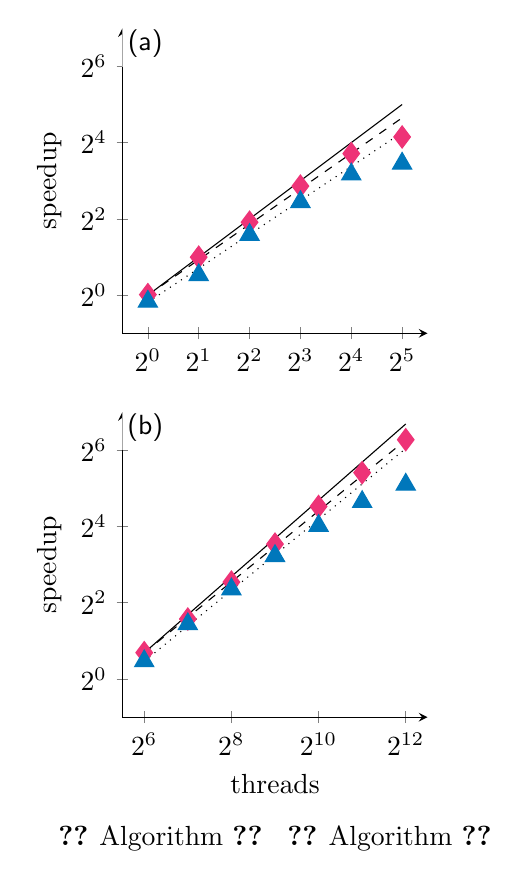
\begin{tikzpicture}
\begin{groupplot}[
    group style={group name=unst-strong, group size=1 by 2},
    width=0.45\textwidth
]
\nextgroupplot[
        xmin=0.70710678118,  % approx. 1/√2
        xmax=45.2548339959,  % approx 32√2
        xmode=log,
        log basis x=2,
        ymode=log,
        ymin=0.5,
        ymax=128,
        log basis y=2,
        log origin=infty,
        width=0.45\textwidth,
        height=0.45\textwidth,
        axis lines=center,
        ylabel={speedup},
        xlabel near ticks,
        ylabel near ticks,
        xtick={1, 2, 4, 8, 16, 32},
        ytick={1, 4, 16, 64},
        legend style={at={(0.5, 0.9)}, anchor=center, draw=none,
                      /tikz/every even column/.append style={column sep=5pt}},
        legend cell align={left},
        legend columns=1
    ]
    \addplot+[only marks, mark=diamond*, color=tol/vibrant/magenta, mark options={scale=2, fill=tol/vibrant/magenta}] coordinates {%
        (1 , {1.30763/1.29442})
        (2 , {1.30763/0.65481})
        (4 , {1.30763/0.34712})
        (8 , {1.30763/0.18004})
        (16, {1.30763/0.09969})
        (32, {1.30763/0.07371})
    }; \label{plot:unst-strong-interp}
    \addplot+[only marks, mark=triangle*, color=tol/vibrant/blue, mark options={scale=2, fill=tol/vibrant/blue}] coordinates {%
        (1 , {1.33840/1.50377})
        (2 , {1.33840/0.92804})
        (4 , {1.33840/0.44697})
        (8 , {1.33840/0.24580})
        (16, {1.33840/0.14895})
        (32, {1.33840/0.12225})
    }; \label{plot:unst-strong-spread}
    \addplot+[no marks, dashed, black, domain=1:32] {x^0.93};
    \addplot+[no marks, dotted, black, domain=1:32] {0.88*x^0.89};
    \addplot+[no marks, black, domain=1:32] {x};
    \node[fill=white] at (rel axis cs: 0.075, 0.95) {\sffamily(a)};
\nextgroupplot[
        xmin=45.2548339959,  % approx 32√2
        xmax=5792.61875148,  % approx 4096√2
        xmode=log,
        log basis x=2,
        ymode=log,
        ymin=0.5,
        ymax=128,
        log basis y=2,
        log origin=infty,
        width=0.45\textwidth,
        height=0.45\textwidth,
        axis lines=center,
        xlabel={threads},
        ylabel={speedup},
        xlabel near ticks,
        ylabel near ticks,
        ytick={1, 4, 16, 64},
        legend style={at={(0.5, 0.9)}, anchor=center, draw=none,
                      /tikz/every even column/.append style={column sep=5pt}},
        legend cell align={left},
        legend columns=1
    ]
    
    \addplot+[only marks, mark=diamond*, color=tol/vibrant/magenta, mark options={scale=2, fill=tol/vibrant/magenta}] coordinates {%
        (64  , {1.30763/0.80977})
        (128 , {1.30763/0.43929})
        (256 , {1.30763/0.22434})
        (512 , {1.30763/0.11258})
        (1024, {1.30763/0.05681})
        (2048, {1.30763/0.03074})
        (4096, {1.30763/0.01689})
    };
    \addplot+[only marks, mark=triangle*, color=tol/vibrant/blue, mark options={scale=2, fill=tol/vibrant/blue}] coordinates {%
        (64  , {1.33840/0.96698})
        (128 , {1.33840/0.49359})
        (256 , {1.33840/0.26208})
        (512 , {1.33840/0.14286})
        (1024, {1.33840/0.08252})
        (2048, {1.33840/0.05351})
        (4096, {1.33840/0.03905})
    };
    \addplot+[no marks, dashed, black, domain=64:4096] {1.61*(x/64)^0.93};
    \addplot+[no marks, dotted, black, domain=64:4096] {1.38*(x/64)^0.93};
    \addplot+[no marks, black, domain=64:4096] {1.61*x/64};
    \node[fill=white] at (rel axis cs: 0.075, 0.95) {\sffamily(b)};
\end{groupplot}
\path (unst-strong c1r2.south west|-current bounding box.south)--
coordinate(legendpos) (unst-strong c1r2.south east|-current bounding box.south);
\matrix[
    matrix of nodes,
    anchor=north,
    inner sep=0.2em,
    %draw
  ]at([yshift=-1ex]legendpos)
  {
    \ref{plot:unst-strong-interp}& Algorithm \ref{algo:par-interp}&[5pt]
    \ref{plot:unst-strong-spread}& Algorithm \ref{algo:otf-spread}\\};
\end{tikzpicture}
\caption{%
Strong scaling results for Algorithm \ref{algo:otf-spread} and grid spacing
$h = 0.5\um$ (a grid refinement of 64) for $2^{16}$ randomly placed IB points
in a $16\um\times16\um\times16\um$ triply periodic domain for (a) 1-32 CPU
cores, and (b) 64-4096 threads on the GPU. Speedup is measured relative to
serial Algorithms \ref{algo:par-interp} and \ref{algo:serial-spread}. The solid
black lines show the trendline for ideal speedup. The dashed or dotted lines
give the initial trend for interpolation and spreading, respectively.
}
\label{fig:unstructured-strong}
\end{figure}

Figure \ref{fig:unstructured-strong} shows the results of these tests. Speedup is
measured relative to the serial interpolation and spreading implementations.  The
trendlines estimate that increasing computing resources by a factor of two decreases
runtime by a factor of about 1.91 for CPU and GPU interpolation and by a factor of about
1.85 for CPU spreading. It is not trivial to limit the number of threads used by
{\thrust} for work done on the GPU, so the key-value sort and segmented reduce use as
many threads as {\thrust} decides is prudent.  While the trendline indicates a decrease
in runtime by a factor of 1.91 as well, this is merely an approximation.  

Parallel CPU interpolation using a single processor is identical to the serial
CPU interpolate, so the CPU interpolate passes through $(1,\,1)$. The same is
not true of parallel spreading using a single processor compared to serial
spreading. Because of the additional sort step in the parallel spreading
algorithm, single-threaded Algorithm \ref{algo:par-spread} is about 12\% slower
than its serial counterpart. The CPU code also enjoys the benefit of using
vector registers for some of the computation. The GPU requires 64 threads to
match the speed of a single CPU core.
%Based on the trendline in Figure
%\ref{fig:unstructured-strong} and the speedup for grid refinement shown in
%Figure \ref{fig:grid-dependence}, we see that the GPU attains a speedup of
%approximately 5.25$\times$ compared to 32 CPU processors, and uses
%approximately 4480 threads, where the kernel reaches the limit on register
%memory.
%
Even at 4096 threads, interpolate on the GPU shows no indication of plateauing. The final
data point for that curve shows a speedup of approximately $77\times$. Figure
\ref{fig:grid-dependence}(b), on the other hand, shows that the maximum speedup we can
expect for this problem is approximately 85$\times$, which the trendline in Figure
\ref{fig:unstructured-strong}(b) predicts will occur at approximately 4480 threads. Thus,
we can expect the plateau for interpolate on the GPU to be very abrupt. This indicates a
hardware limitation, the likely culprit being exhaustion of register memory. The
plateauing of the CPU curves is not a limitation of the algorithm for the CPU. Despite
having 48 cores, the test using 32 cores did not utilize them at full capacity. Using
fewer cores, on the other hand, was able to maintain full utilization for the duration of
the test. If not for having a comparatively limited number of CPU cores, we expect to see
the CPU trend continue.

If not for hardware limitations, it seems that the algorithm scales without bound on
either the CPU of GPU. Overall, trends for the CPU and GPU are very similar. Because of
these similarities, we will restrict ourselves to the GPU, but expect any conclusions to
hold for the CPU as well.

\subsubsection{Weak scaling}\label{sec:unst-weak}
In contrast, with improved computing resources, we may wish to solve bigger problems. The
ideal parallel algorithm solves a problem with $p$ threads in the same time as it solves
a twice bigger problem with $2p$ threads. Here, we place between $2^{16}$ and $2^{19}$
points randomly in the domain. We increase the number of threads proportionally, between
128 and 1024.  

\begin{table}[ht]
    \begin{center}
        \begingroup
        \setlength{\tabcolsep}{9pt}
        \renewcommand{\arraystretch}{1.5}
%        \begin{tabular}{ccccc}
%                                                                                               \toprule
%            $p$  & $n$      & \titletable{interpolate}{20000}  & \titletable{spread}{10000} \\ \midrule
%            128  & $2^{16}$ & $0.43930 \pm 0.00372 $           & $0.47632 \pm 0.00278 $     \\
%            256  & $2^{17}$ & $0.44918 \pm 0.01097 $           & $0.46503 \pm 0.00050 $     \\
%            512  & $2^{18}$ & $0.45072 \pm 0.01195 $           & $0.44533 \pm 0.00054 $     \\
%            1024 & $2^{19}$ & $0.45442 \pm 0.00960 $           & $0.43561 \pm 0.00047 $     \\ \bottomrule
%        \end{tabular}
        \begin{tabular}{ccccc}
                                                                                               \toprule
            $p$  & $n$      & \titletable{interpolate}{20000} & \titletable{spread}{10000} \\ \midrule
            128  & $2^{16}$ & $0.43930$                       & $0.47632$                  \\
            256  & $2^{17}$ & $0.44918$                       & $0.46503$                  \\
            512  & $2^{18}$ & $0.45072$                       & $0.44533$                  \\
            1024 & $2^{19}$ & $0.45442$                       & $0.43561$                  \\ \bottomrule
        \end{tabular}                                                                                             \endgroup
    \end{center}
    \caption{%
Weak scaling results for interpolation and spreading for $p$ threads and $n$ randomly
placed IB points in a $16\um\times16\um\times16\um$ triply periodic domain with
$h=0.5\um$ on the GPU. 
%95\% confidence intervals for average time per call are reported
Average time per call is reported
in seconds. $N$ is the number of samples taken.
    }
    \label{tab:unstructured-weak}
\end{table}

Table \ref{tab:unstructured-weak} lists runtimes for increasing threads and
problem size on the GPU. Interpolate scales nearly perfectly with a difference
of $15\ms$ (\textasciitilde3\%) increase between the problem with 128 threads
and $2^{16}$ IB points and that with 1024 threads and $2^{19}$ points. Spread,
on the other hand, decreases in time as the problem size increases. This
speedup is artificial, and should not be expected in general. In the $n=2^{16}$
case, there is 1 IB point for every 4 grid cells, on average. When $n=2^{19}$,
the density increases to 2 for every grid cell. As a result, it becomes
increasingly unlikely to find a cell containing no IB points. This means that
writing the values to the output vector(s) becomes increasingly coalesced,
which, in turn, reduces the number of writes to global memory and vastly
improves the speed of the write overall. Typical use of the IB method does not
have IB points in every grid cell, but the recommendations that IB points on
connected structures be spaced $0.5h$--$h$ apart typically yields 1--4 IB
points in each occupied grid cell. We now consider a more typical use of the IB
method.

% vim: cc=90 tw=89


\subsection{Elastic Objects}

We are motivated by the desire to simulate the motion of cells immersed in a fluid. Cells
are not randomly generated points, but cohesive structures, kept together by elastic
forces and the near-constant volume enclosed by their membranes. In this section, we
replace the randomly-placed IB points with points sampled on the surface of either a
sphere or an RBC. We track $n_d$ data sites per object, and interpolate fluid velocities
only to these points. We construct an RBF interpolant based on the positions of the data
sites and evaluate forces at $n_s$ sample sites, chosen so that neighboring sample sites
are initially within approximately $0.5h$ of each other. We spread forces from the sample
sites. It is generally the case that $n_s > n_d$, so that we interpolate to fewer points
than we spread from. In the parlance of Section \ref{sec:parallel}, $n_\gamma=n_d$ in the
context of interpolation, and $n_\gamma=n_s$ in the context of spreading. These point
sets are generated by the \texttt{KernelNode} library. In this case, we invoke the fluid
solver, so that as the object deforms, the force it imparts on the fluid will affect the
fluid velocity. The sphere and RBC are elastic, obeying the Skalak constitutive law
\cite{Skalak:1973tp} with shear modulus $2.5\times10^{-3}\dynpercm$ and bulk modulus
$2.5\times10^{-1}\dynpercm$. The RBC has rest configuration given in \cite{Omori:2012hw}:
\begin{equation}
    \begin{aligned}
        x(\theta,\,\varphi) &= R_0\cos\theta\cos\varphi, \\
        y(\theta,\,\varphi) &= R_0\sin\theta\cos\varphi, \\
        z(\theta,\,\varphi) &= \sfrac12 R_0\sin\varphi\left[0.21 + 2.0 \cos^2\varphi -1.12 \cos^4\varphi\right],
    \end{aligned}
\end{equation}
where $R_0=3.91\um$, $\theta\in[-\pi,\,\pi)$, and $\varphi\in[-\pi/2,\,\pi/2]$. These
tests require a timestep of $k=0.1\us$ for stability. With $\shear=1000\si{\per\second}$,
an IB point requires at least 32 timesteps to transit a grid cell, so unlike the tests
using randomly placed IB points above, there will be considerably more redundant
computation. We first validate the fluid solver with the elastic sphere before performing
scaling tests, similar to those above, with RBCs.

\subsubsection{Convergence study}
To test the convergence of the fluid solver and cell representation, consider 
an object that obeys Skalak's law with the coefficients given above and is
spherical at rest. Deform the object from its rest configuration by stretching
it by a factor of $1.1$ in the $z$ direction and compressing it by a factor of
$1.1$ in the $y$ direction to maintain a fixed volume. For this test, $\shear$
is zero, so the fluid velocity is intially zero, and the object tends toward
its rest configuration over the course of simulation. We allow the object to
relax for $16\us$, and compare errors generated by successive grid refinements
of 16, 32, 64, and 128 points per $16\um$. For each grid, we use a fixed set of
$n_d=625$ data sites, sampled approximately uniformly on the surface of the
sphere, and choose $n_s$ so that sample sites are approximately uniform and
roughly $h/1.1$ apart, so that sample sites are roughly $h$ apart initially.
For $h=1\um$, $n_s=220$, and a refinement by a factor of 2 increases $n_s$ by a
factor of 4, for a maximum number of 14080 sample sites for these tests. A thin
interface which generates a force will cause a jump in the normal stress across
the interface, which the IB method may not recover. We therefore anticipate
first order convergence for the fluid velocity and data site positions.

\begin{table}
    \begin{center}
        \begingroup
        \setlength{\tabcolsep}{9pt}
        \renewcommand{\arraystretch}{1.5}
        \begin{tabular}{cc|cc|cc}
                                                                                                                 \\ \toprule
            $h$       & $k$       & $\|\u_h-\u_{0.5h}\|_2$ & order    & $\|\u_h-\u_{0.5h}\|_{\infty}$ & order    \\ \midrule
            $1.00\um$ & $1.6\us$ & $2.22736\times10^{-2}$ &          & $7.41870\times10^{-2}$        &          \\
            $0.50\um$ & $0.4\us$ & $4.32802\times10^{-4}$ & 5.715132 & $1.90832\times10^{-3}$        & 5.280787 \\
            $0.25\um$ & $0.1\us$ & $1.46835\times10^{-4}$ & 1.559507 & $1.08472\times10^{-3}$        & 0.814971 \\ \bottomrule
        \end{tabular}
        \endgroup
    \end{center}
    \caption{%
Convergence of the fluid velocity for a deformed sphere returning to its rest
configuration in a $16\um\times16\um\times16\um$ triply periodic domain at
$t=160\us$. The finest grid, with $h=0.125\um$ uses timestep $k=0.025\us$.
    }
    \label{tab:u-convergence}
\end{table}

\begin{table}
    \begin{center}
        \begingroup
        \setlength{\tabcolsep}{9pt}
        \renewcommand{\arraystretch}{1.5}
        \begin{tabular}{cc|cc|cc}
                                                                                                             \\ \toprule
            $h$       & $n_s$ & $\|\X_h-\X_{0.5h}\|_2$ & order    & $\|\X_h-\X_{0.5h}\|_{\infty}$ & order    \\ \midrule
            $1.00\um$ & 220   & $2.96106\times10^{-3}$ &          & $4.78122\times10^{-3}$        &          \\
            $0.50\um$ & 880   & $7.29973\times10^{-4}$ & 2.020201 & $1.16865\times10^{-3}$        & 2.032531 \\
            $0.25\um$ & 3520  & $3.59088\times10^{-4}$ & 1.023507 & $6.09555\times10^{-4}$        & 0.939021 \\ \bottomrule
        \end{tabular}
        \endgroup
    \end{center}
    \caption{%
Convergence of data sites for a deformed sphere returning to its rest
configuration in a $16\um\times16\um\times16\um$ triply periodic domain at
$t=16\us$. For each grid, we track 625 data sites on the sphere. The finest
grid, with $h = 0.125\um$ used $n_s=14080$ sample sites.
    }
    \label{tab:x-convergence}
\end{table}

Tables \ref{tab:u-convergence} and \ref{tab:x-convergence} show the convergence
of fluid velocity and data sites, respectively. To compute errors in the fluid
velocity, we construct a cubic spline from the velocities on the finer grid
and evaluate the spline at the grid points of the coarser grid. Each of the
interfaces is constructed with the same number of data sites, so the
coordinates from one simulation to another can be compared directly. We recover
approximately first order convergence for both fluid velocity and data sites
positions. Having established asymptotic convergence of our IB solver, we
continue by performing scaling tests with RBCs.

\subsubsection{Strong scaling}

We again wish to see how these algorithms can help speed up the runtime of
a fixed problem. Here, we consider tests with a single RBC and with 4 RBCs.
To construct the RBCs, we now use $n_d=864$ data sites, for an initial data
site spacing of approximately $1.6h$, and $n_s=8832$ sample sites per cell, for
an initial sample site spacing of approximately $0.5h$. We use a timestep of
$k=0.1\us$ to simulate the motion of the cells for $1\ms$.

%\begin{table}
%    \begin{center}
%        \begingroup
%        \setlength{\tabcolsep}{9pt}
%        \renewcommand{\arraystretch}{1.5}
%        \begin{tabular}{ccccc}
%            $p$  & cells & \titletable{interpolate}{20000} & \titletable{spread}{10000} \\ \hline
%%            1    & 1     & $0.47633 \pm 0.00024$           & $4.58460 \pm 0.00821$      \\
%%            2    & 1     & $0.26608 \pm 0.00146$           & $2.59113 \pm 0.00567$      \\
%%            4    & 1     & $0.14505 \pm 0.00080$           & $1.44780 \pm 0.00353$      \\
%%            8    & 1     & $0.07593 \pm 0.00031$           & $0.76037 \pm 0.00229$      \\
%%            16   & 1     & $0.04010 \pm 0.00009$           & $0.40348 \pm 0.00137$      \\
%%            32   & 1     & $0.02037 \pm 0.00007$           & $0.22602 \pm 0.00105$      \\
%            64   & 1     & $0.01080 \pm 0.00004$           & $0.11888 \pm 0.00055$      \\
%            128  & 1     & $0.00586 \pm 0.00002$           & $0.06535 \pm 0.00023$      \\
%            256  & 1     & $0.00341 \pm 0.00002$           & $0.03912 \pm 0.00012$      \\
%            512  & 1     & $0.00179 \pm 0.00001$           & $0.02649 \pm 0.00014$      \\
%            1024 & 1     & $0.00093 \pm 0.00001$           & $0.01924 \pm 0.00011$      \\
%            2048 & 1     & $0.00094 \pm 0.00001$           & $0.01627 \pm 0.00012$      \\
%            4096 & 1     & $0.00093 \pm 0.00001$           & $0.01455 \pm 0.00009$%      \\
%%            8192 & 1     & $0.00094 \pm 0.00001$           & $0.01413 \pm 0.00010$
%        \end{tabular}
%        \endgroup
%    \end{center}
%    \caption{%
%        Results of strong scaling tests for IB spreading and interpolate.
%        Reported values are in seconds.
%    }
%\end{table}

\begin{figure}[ht]
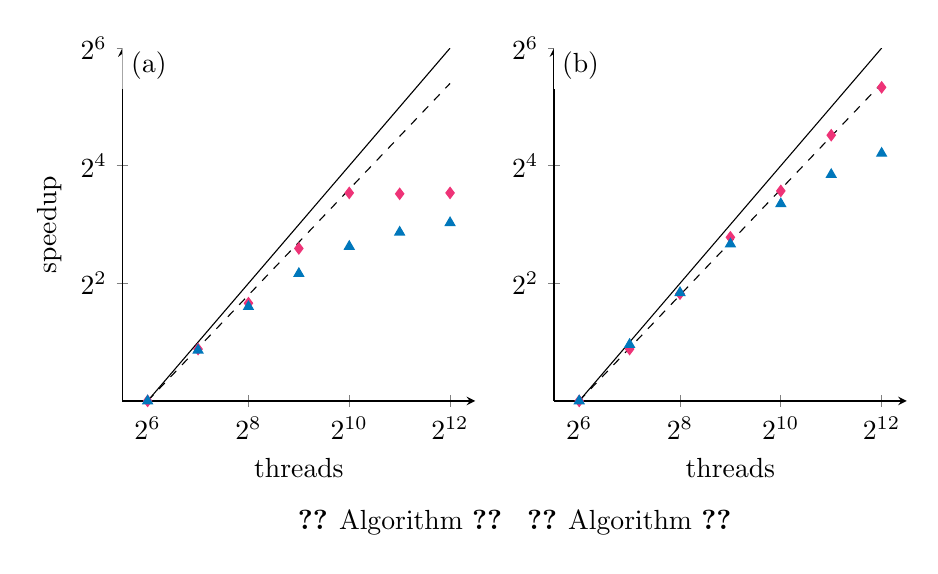
\begin{tikzpicture}
\begin{groupplot}[
    group style={group name=rbc-strong, group size=2 by 1},
    height=0.5\textwidth,
    width=0.5\textwidth
]
\nextgroupplot[
        xmode=log,
        xmin=45.2548339959,
        xmax=5792.61875148,
        log basis x=2,
        ymode=log,
        ymax=64,
        log basis y=2,
        log origin=infty,
        width=0.5\textwidth,
        height=0.5\textwidth,
        axis lines=center,
        xlabel={threads},
        ylabel={speedup},
        xlabel near ticks,
        ylabel near ticks,
        legend style={at={(0.8, 0.2)}, anchor=center},
        legend cell align={left}
]
    \addplot+[only marks, mark=diamond*, color=tol/vibrant/magenta, mark options={fill=tol/vibrant/magenta}] coordinates {%
        (64  , {0.01080/0.01080})
        (128 , {0.01080/0.00586})
        (256 , {0.01080/0.00341})
        (512 , {0.01080/0.00179})
        (1024, {0.01080/0.00093})
        (2048, {0.01080/0.00094})
        (4096, {0.01080/0.00093})
    }; \label{plot:rbc-interp}
    \addplot+[only marks, mark=triangle*, color=tol/vibrant/blue, mark options={fill=tol/vibrant/blue}] coordinates {%
        (64  , {0.11888/0.11888})
        (128 , {0.11888/0.06535})
        (256 , {0.11888/0.03912})
        (512 , {0.11888/0.02649})
        (1024, {0.11888/0.01924})
        (2048, {0.11888/0.01627})
        (4096, {0.11888/0.01455})
    }; \label{plot:rbc-spread}
    \addplot+[no marks, dashed, black, domain=64:4096] {(x/64)^0.9};
    \addplot+[no marks, black, domain=64:4096] {(x/64)};
    \node [fill=white] at (rel axis cs: 0.075, 0.95) {(a)};
\nextgroupplot[
        xmode=log,
        xmin=45.2548339959,
        xmax=5792.61875148,
        log basis x=2,
        ymode=log,
        ymax=64,
        log basis y=2,
        log origin=infty,
        width=0.5\textwidth,
        height=0.5\textwidth,
        axis lines=center,
        xlabel={threads},
        xlabel near ticks,
        ylabel near ticks,
        legend style={at={(0.8, 0.2)}, anchor=center},
        legend cell align={left}
    ]
    \addplot+[only marks, mark=diamond*, color=tol/vibrant/magenta, mark options={fill=tol/vibrant/magenta}] coordinates {%
        (64  , {0.04150/0.04150})
        (128 , {0.04150/0.02251})
        (256 , {0.04150/0.01172})
        (512 , {0.04150/0.00603})
        (1024, {0.04150/0.00349})
        (2048, {0.04150/0.00181})
        (4096, {0.04150/0.00103})
    };
    \addplot+[only marks, mark=triangle*, color=tol/vibrant/blue, mark options={fill=tol/vibrant/blue}] coordinates {%
        (64  , {0.40148/0.40148})
        (128 , {0.40148/0.20628})
        (256 , {0.40148/0.11208})
        (512 , {0.40148/0.06313})
        (1024, {0.40148/0.03931})
        (2048, {0.40148/0.02785})
        (4096, {0.40148/0.02168})
    };
    \addplot+[no marks, dashed, black, domain=64:4096] {(x/64)^0.9};
    \addplot+[no marks, black, domain=64:4096] {(x/64)};
    \node [fill=white] at (rel axis cs: 0.075, 0.95) {(b)};
\end{groupplot}
\path (rbc-strong c1r1.south west|-current bounding box.south)--
coordinate(legendpos) (rbc-strong c2r1.south east|-current bounding box.south);
\matrix[
    matrix of nodes,
    anchor=north,
    inner sep=0.2em,
    %draw
  ]at([yshift=-1ex]legendpos)
  {
      \ref{plot:rbc-interp}& Algorithm \ref{algo:par-interp}&[5pt]
      \ref{plot:rbc-spread}& Algorithm \ref{algo:otf-spread} \\};
\end{tikzpicture}
\caption{%
    Speedup of Algorithms \ref{algo:par-interp} and \ref{algo:otf-spread} with
    increasing numbers of threads compared to 64 threads on the GPU for (a) 1
    and (b) 4 RBCs. Speedup is measured relative to the time taken for each
    algorithm using 64 threads on the GPU. Dashed lines indicate trends, and
    solid lines indicate ideal scaling.
}
\label{fig:str-strong}
\end{figure}

Figure \ref{fig:str-strong} shows the speedup observed with increasing threads
for 1 and 4 RBCs for 64--4096 threads on the GPU. We again see that the initial
speedup for interpolation is nearly linear with increased threads. In subfigure
\ref{fig:str-strong}(a), there is a sharp plateau that corresponds to every
data site having its own thread. In other words, there are more threads than
there is work to be done, since we track only 864 data sites for a single RBC.
Subfigure \ref{fig:str-strong}(b), on the other hand, has 3456 data sites, so
the trend continues for 512--4096 threads. In this case, we expect this graph
to plateau beyond 4096, when each data site has its own thread. However, we do
not expect for the trend to continue with more cells, as the presumed maximum
number of threads for interpolation is 4480, as discussed in Section
\ref{sec:unst-strong}. Comparing subfigure \ref{fig:str-strong}(a)
to (b), we see that the speedup in spreading is also dependent on the amount of
work. This indicates that, as with interpolation, the maximum speedup for
spreading is limited by hardware, rather than being a limitation of the
algorithm.

The trendlines for these tests indicate that increasing computing resources
by a factor of two decreases runtime by a factor of about 1.87 for these
algorithms. Again, this is merely an approximation as the sort and reduction
steps of the spreading algorithm are provided by {\thrust}, and therefore are
not limited to the listed number of threads. The similarity between the result
of the tests with RBCs and with randomly placed points indicates that the
distribution of points does not have a marked impact on the efficacy of the
parallelization for a fixed problem. We now see if the same holds for weak
scaling tests.


%\begin{table}
%    \begin{center}
%        \begingroup
%        \setlength{\tabcolsep}{9pt}
%        \renewcommand{\arraystretch}{1.5}
%        \begin{tabular}{ccccc}
%            $p$   & cells & \titletable{interpolate}{20000} & \titletable{spread}{10000} \\ \hline
%            64    & 4     & $0.04150 \pm 0.00013$           & $0.40148 \pm 0.00146$      \\
%            128   & 4     & $0.02251 \pm 0.00003$           & $0.20628 \pm 0.00060$      \\
%            256   & 4     & $0.01172 \pm 0.00002$           & $0.11208 \pm 0.00031$      \\
%            512   & 4     & $0.00603 \pm 0.00002$           & $0.06313 \pm 0.00014$      \\
%            1024  & 4     & $0.00349 \pm 0.00002$           & $0.03931 \pm 0.00011$      \\
%            2048  & 4     & $0.00181 \pm 0.00001$           & $0.02785 \pm 0.00011$      \\
%            4096  & 4     & $0.00103 \pm 0.00001$           & $0.02168 \pm 0.00009$
%        \end{tabular}
%        \endgroup
%    \end{center}
%    \caption{%
%        Results of strong scaling tests for IB spreading and interpolate with
%        4 RBCs.
%        Reported values are in seconds.
%    }
%\end{table}

\subsection{Weak scaling of interaction operations}

\begin{table}
    \begin{center}
        \begingroup
        \setlength{\tabcolsep}{9pt}
        \renewcommand{\arraystretch}{1.5}
        \begin{tabular}{ccccc}
            $p$ & cells & \titletable{interpolate}{20000} & \titletable{forces}{10000} & \titletable{spread}{10000} \\ \hline
            64  & 1     & $0.01079 \pm 0.00004$           & $0.00242 \pm 0.00002$      & $0.11881 \pm 0.00055$      \\
            128 & 2     & $0.01165 \pm 0.00003$           & $0.00249 \pm 0.00002$      & $0.11219 \pm 0.00051$      \\
            256 & 4     & $0.01171 \pm 0.00003$           & $0.00287 \pm 0.00003$      & $0.11214 \pm 0.00036$      \\
            512 & 8     & $0.01199 \pm 0.00003$           & $0.00532 \pm 0.00008$      & $0.11354 \pm 0.00047$
        \end{tabular}
        \endgroup
    \end{center}
    \caption{%
        Weak scaling results.
    }
\end{table}

\begin{table}
    \begin{center}
        \begingroup
        \setlength{\tabcolsep}{9pt}
        \renewcommand{\arraystretch}{1.5}
        \begin{tabular}{ccccc}
            $p$  & $n$      & \titletable{interpolate}{20000} & \titletable{forces}{10000} & \titletable{spread}{10000} \\ \hline
            128  & $2^{16}$ & $0.43930 \pm 0.00019$           & $0.00026 \pm 0.00031$      & $0.47632 \pm 0.00142$      \\
            256  & $2^{17}$ & $0.44918 \pm 0.00056$           & $0.00024 \pm 0.00002$      & $0.46503 \pm 0.00026$      \\
            512  & $2^{18}$ & $0.45072 \pm 0.00061$           & $0.00029 \pm 0.00001$      & $0.44533 \pm 0.00028$      \\
            1024 & $2^{19}$ & $0.45442 \pm 0.00049$           & $0.00055 \pm 0.00000$      & $0.43561 \pm 0.00024$      \\
        \end{tabular}
        \endgroup
    \end{center}
    \caption{%
        Results of $n$ randomly placed IB points in a 16 \si{\micro\meter}
        $\times$ 16 \si{\micro\meter} $\times$ 16 \si{\micro\meter} periodic
        domain.
    }
\end{table}


% vim: cc=90 tw=89

\section{Summary}

We have presented a parallel algorithm for interpolation and introduced a novel parallel
algorithm for spreading forces from time-dependent interfaces in the immersed boundary
method. These algorithms have a runtime that is independent of the Eulerian grid. This
makes the parallelization useful for cases where IB points inhabit only a small
percentage of the Eulerian grid cells. We have also introduced two variants for spread
which trade off dependence on the Eulerian grid, in the form of a few vector adds and
memory allocation, for improved runtimes for small enough grids.

These algorithms exhibit nearly ideal scaling, on both the CPU and GPU, for problems of
fixed size and increasing number of threads, as well as for problems of increasing size
and number of threads.  We observed that on the GPU, larger problem sizes led to higher
speedup plateaus, indicating that larger problems on more capable hardware will achieve
even larger speedups than presented here.

% vim: cc=90 tw=89


%\begin{acknowledgements}
%\end{acknowledgements}


% Authors must disclose all relationships or interests that 
% could have direct or potential influence or impart bias on 
% the work: 
%

%\section*{Conflict of interest}


\bibliographystyle{spmpsci}      % mathematics and physical sciences
\end{document}
% end of file template.tex

